\documentclass[10pt]{beamer}
%\documentclass[handout,10pt]{beamer}

\mode<presentation>
{
\usetheme{PI}
}

\usepackage[utf8]{inputenc}
\usepackage[english]{babel}
\usepackage{etex}
\usepackage{listings}
\usepackage{pstricks-add}
\usepackage{url}					
\usepackage{booktabs}			
\usepackage{dcolumn}			
\usepackage{bm}						
\usepackage[left]{eurosym}
\usepackage{subfigure}		
\usepackage{color}				
\usepackage{epstopdf}	
\usepackage[absolute,overlay]{textpos} 
\usepackage{multirow}
\usepackage{textpos}
\usepackage{tikz}
\usepackage{pst-pdf}
\usepackage{graphicx}
\usepackage{pgfpages}

\lstset{
    language=XML,
    keywordstyle=\bfseries\ttfamily\color{blue},
    identifierstyle=\ttfamily\color{black},
    commentstyle=\color[rgb]{0.457,0.723,0.0},
    stringstyle=\ttfamily\color[rgb]{0.627,0.126,0.941},
    showstringspaces=false,
    basicstyle=\scriptsize,
    numberstyle=\scriptsize,
    numbers=left,
    stepnumber=1,
    numbersep=4pt,
    tabsize=2,
    breaklines=true,
    keepspaces=true,
    breakatwhitespace=false,
    aboveskip={1.5\baselineskip},
    columns=flexible,
    frame=single key,
    captionpos=b,
    morekeywords={name,class,threshold,weight,parameter}
    }

%Create Handout?
\only<handout>{\pgfpagesuselayout{4 on 1}[a4paper,landscape]}

%Use BeamerNotes?
%\setbeameroption{show notes on second screen=right}
\graphicspath{{images/}}

\title[SiLift]{High-level Differencing, Patching and Merging of EMF Models}
%\subtitle{SubTitle}
\author[D. Reuling \\ M. Ohrndorf]{Dennis Reuling -- Manuel Ohrndorf}
\date[18.11.2013]{Eclipse DemoCamp}
\pgfdeclareimage[height=1.5cm]{titlegraphic}{logoTitle}
\titlegraphic{\pgfuseimage{titlegraphic}}

\hypersetup{
	pdfauthor={Dennis Reuling, Manuel Ohrndorf},
    pdfsubject={SiLift: High-level Differencing, Patching and Merging of EMF Model}
	pdfkeywords={SiLift, EMF Compare, Differences, Operations, Lifting, Patching,
	Merging} }

%\beamerdefaultoverlayspecification{<+$\rightarrow$}

\begin{document}

 \pgfdeclareverticalshading{fadeBlue}{\paperwidth}%
 {color(0cm)=(bg);color(1cm)=(structure.fg!25!structure.bg)}

\begingroup
\makeatletter
%\setbeamertemplate{background canvas}[vertical shading][top=bg,bottom=structure.fg!25!structure.bg]
\only<presentation>{\setlength{\hoffset}{-25pt}}
\beamertemplatenavigationsymbolsempty
\makeatother
\begin{frame}[plain]
    \titlepage
\end{frame}
\endgroup

%no subsections in toc
\setcounter{tocdepth}{1}

\begingroup
\makeatletter
\setbeamertemplate{sidebar left}{}
\makeatother
\begin{frame}
\frametitle{About us}
\begin{block}{Software Engineering Group, University of Siegen}
Main research area: Model Driven Software Development \\
\medskip
\textbf{Web:} \url{http://pi.informatik.uni-siegen.de}
\end{block}
\begin{block}{Dennis Reuling, M. Sc.}
Research Scientist at SEG\\
%\medskip
%\textbf{Thesis:} Integration of UML Profiles into the SiDiff and SiLift tools
% based on a SysML case study \\
\medskip
\textbf{Email:} \url{dreuling@informatik.uni-siegen.de}

\end{block}
\begin{block}{Christopher Pietsch}
Research Assistant at SEG \\
%\medskip
%\textbf{Thesis:} Generation of transformation rules for the optimization of
% model differences\\
\medskip
\textbf{Email:} \url{cpietsch@informatik.uni-siegen.de}
\end{block}
\end{frame}
\endgroup

\begingroup
\makeatletter
\setbeamertemplate{sidebar left}{}
\makeatother
\begin{frame}
  \frametitle{Agenda}
  \tableofcontents
\end{frame}
\endgroup

\AtBeginSection[]%
{%
\frame{\sectionpage}
}

\chapter*{Introduction}\label{introduction}
The paradigm shift from coding to modeling can easily be called one of the
biggest changes in progress in the area of software development. 
The main reason for this change has been the rising complexity of software,
whether it be in product families, different versions or the software itself.
Developers are trying to restrain this complexity by using modeling languages
and tools, which focus on the semantics of the given problem instead of
underlying programming languages.
Elevating the abstraction level eases the understanding of the problem and can
be one solution to cope with the rising complexity of software.

One important aspect to facilitate this paradigm shift is the definition of
modeling languages conforming to problems in practical domains of software. The
\ac{UML} has been introduced as such general-purpose modeling language and has
been accepted by the \ac{ISO} as industry standard for modeling
software-intensive systems since 2000. Although the modeling language already
supports many areas of software development like \textit{activities} or \textit{data modeling}, the \ac{UML} provides the generic facility for possible adaptions in
new areas or domains via its own \textit{profiling} mechanism: The \ac{UML} or
subsets of it can be extended by declaring own domain specific elements, adding
new properties to already existent modeling elements. The profiling mechanism is defined in an additive manner, therefore all profiled \ac{UML} elements are
still conforming to the \ac{UML} standard. Two popular examples of \ac{UML}
Profiles used by software developers in practice are \ac{SysML} and \ac{MARTE}.

Another important aspect for supporting \ac{MDSD} are the modeling tools
themselves, which should provide all needed and well-known features 
supported by text-based tools. To keep complex software manageable, there has to be the possibility to work in
sufficient large teams in parallel, without giving up the freedom of single
developers. Text-based tools are providing all necessary features for working
in teams since decades like the detection of correspondences and
differences between two revisions of software. The \textit{SiDiff} tool provides
such features for modeling languages: By implementing different
matching services, SiDiff can compute corresponding elements between two models
and is therefore the foundation of supporting parallel work in software
development. The \textit{SiLift} tool takes the support one step further in the
modeling tool pipeline: The detected differences are lifted upon a more
understandable level for the developer by presenting the changes via edit
operations. On this level of abstraction the changes are more comprehensive for
the developer,
which is crucial to parallel work paradigms. In the context of product families another feature is
well known from text-based tools, which has mostly been absent in the modeling
area: Patching of software. By making use of both SiDiff and SiLift another tool
has been developed, which facilitates this functionality in the modeling domain.
By supporting these three functionalities, \textit{Matching}, \textit{Lifting}
and \textit{Patching}, all basic features needed for parallel development are
available in \ac{MDSD}.

Supporting modeling languages, which conform to problems in
practical domains, in modeling tools, which facilitate well-known features in
parallel development areas, is a big step for the paradigm
shift to \ac{MDSD}. This Master's Thesis describes this integration process and
is structured as follows:

\textbf{Chapter \ref{environment_and_tools}} introduces the mentioned
environment consisting of the modeling language \ac{UML} including its profile
mechanism and the tools used for the integration.

\textbf{Chapter \ref{integration}} describes the concepts of the whole
integration process in a detailed manner, considering each pipeline step of the
modeling tools.

\textbf{Chapter \ref{realization}} illustrates the implementation of the
concepts described beforehand, whereas details and problems are
demonstrated.

\textbf{Chapter \ref{sysml}} analyzes a \ac{SysML} case study in a comprehensive
way, which will be used in the following chapter as input for testing the created solutions.

\textbf{Chapter \ref{solution}} sums up the integration success by
testing the solution using the case study described in the preceding chapter.

\textbf{Chapter \ref{conclusionfuturework}} considers the results from all
preceding chapters and presents a possible outlook and future work.



\section{SiLift Tools}
\begin{frame}
\frametitle{Use Case (1)}
\begin{block}{Differencing}
  \begin{center}
\includegraphics[scale=0.5]{images/createPatch}
  \end{center}
\end{block}
\end{frame}
\begin{frame}
  \frametitle{Difference Viewer}
  \begin{center}
 % \includegraphics[scale=0.4]{images/createPatch} \\ 
 % \medskip
  \includegraphics[scale=0.5]{images/symmetric_collapsed}
  \end{center}
\end{frame}
\begin{frame}
\frametitle{Use Case (2)}
\begin{block}{Patching}
  \begin{center}
\includegraphics[scale=0.5]{images/applyPatch}
  \end{center}
\end{block}
\end{frame}
\begin{frame}
  \frametitle{Consistency-Preserving Editing of Patches (1)}
  \begin{center}
 % \includegraphics[scale=0.4]{images/editPatch} \\ 
 % \medskip
  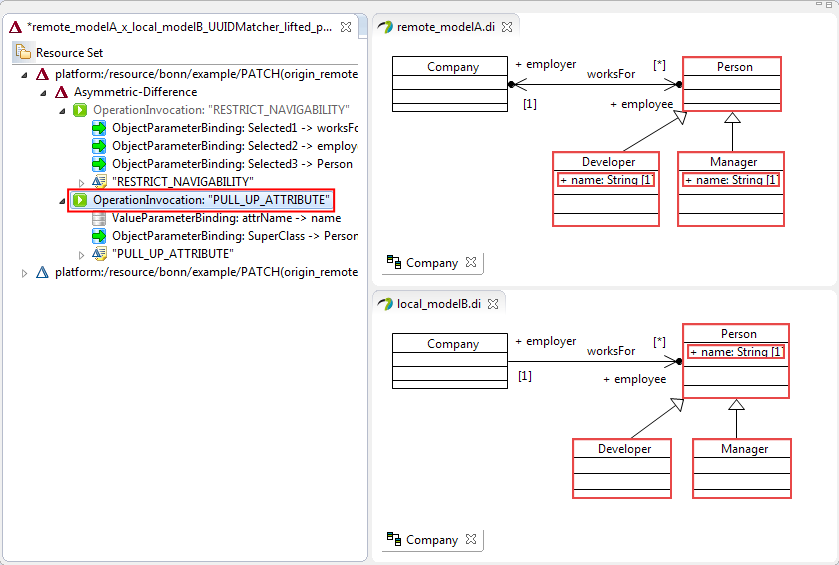
\includegraphics[scale=0.425]{images/asymmetric_pull_up_attribute_1}
  \end{center}
\end{frame}
\begin{frame}[noframenumbering]
  \frametitle{Consistency-Preserving Editing of Patches (2)}
  \begin{center}
 % \includegraphics[scale=0.4]{images/editPatch} \\ 
 % \medskip
  \includegraphics[scale=0.425]{images/asymmetric_pull_up_attribute_2}
  \end{center}
\end{frame}
\begin{frame}
  \frametitle{Controlled Application of Model Patches (1)}
  \begin{center}
 % \includegraphics[scale=0.4]{images/applyPatch} \\ 
 % \medskip
  \includegraphics[scale=0.45]{images/patch_01_1}
  \end{center}
\end{frame}
\begin{frame}[noframenumbering]
  \frametitle{Controlled Application of Model Patches (2)}
  \begin{center}
 % \includegraphics[scale=0.4]{images/applyPatch} \\ 
 % \medskip
  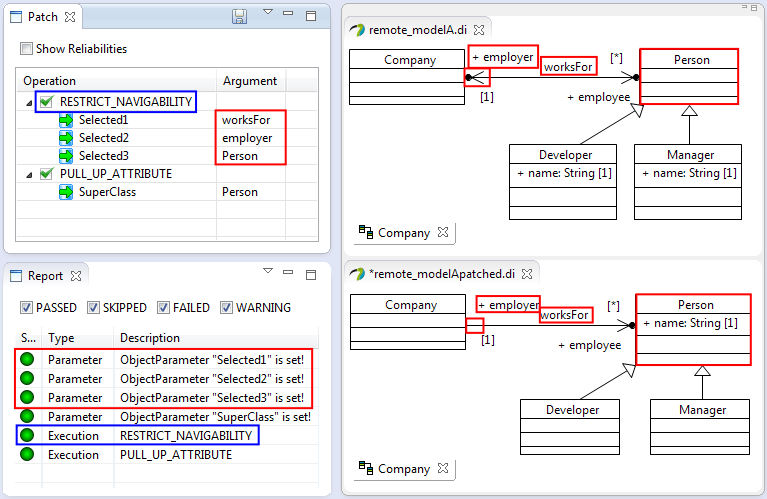
\includegraphics[scale=0.45]{images/patch_01_2}
  \end{center}
\end{frame}
\begin{frame}[noframenumbering]
  \frametitle{Controlled Application of Model Patches (3)}
  \begin{center}
 % \includegraphics[scale=0.4]{images/applyPatch} \\ 
 % \medskip
  \includegraphics[scale=0.45]{images/patch_01_3}
  \end{center}
\end{frame}
\begin{frame}
\frametitle{Use Case (3)}
\begin{block}{Merging}
  \begin{center}
\includegraphics[scale=0.5]{images/applyPatchMerge}
  \end{center}
\end{block}
\end{frame}
\begin{frame}
  \frametitle{Controlled Merging (1)}
  \begin{center}
 % \includegraphics[scale=0.4]{images/applyPatchMerge} \\ 
 % \medskip
  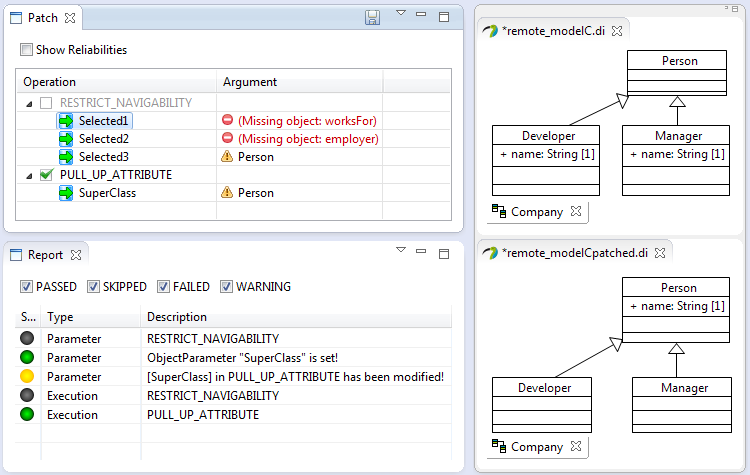
\includegraphics[scale=0.45]{images/patch_02_1}
  \end{center}
\end{frame}
\begin{frame}[noframenumbering]
  \frametitle{Controlled Merging (2)}
  \begin{center}
 % \includegraphics[scale=0.4]{images/applyPatchMerge} \\ 
 % \medskip
  \includegraphics[scale=0.45]{images/patch_02_2}
  \end{center}
\end{frame}
\begin{frame}[noframenumbering]
  \frametitle{Controlled Merging (3)}
  \begin{center}
 % \includegraphics[scale=0.4]{images/applyPatchMerge} \\ 
 % \medskip
  \includegraphics[scale=0.45]{images/patch_02_3}
  \end{center}
\end{frame}
\section{SiLift Approach}

\begin{frame}
  \frametitle{SiLift Pipeline (low level)}
  \begin{center}
  \includegraphics[scale=0.45]{images/pipeline_low-level}
  \end{center}
\end{frame}

\begin{frame}
  \frametitle{SiLift Pipeline (high level)}
  \begin{center}
  \includegraphics[scale=0.45]{images/pipeline_high-level}
  \end{center}
\end{frame}

\begin{frame}
  \frametitle{Theoretical Foundation}
  \begin{center}
  \includegraphics[scale=0.4]{images/graph_theory}
  \end{center}
\end{frame}

\begin{frame}
  \frametitle{Practical Usage}
  \begin{center}
  \includegraphics[scale=2.0]{images/henshinLogo}\\
  \includegraphics[scale=0.3]{images/pullUp_HR}
  \end{center}
\end{frame}
\section{Summary}
\begin{frame}
  \frametitle{Summary}  
  \begin{itemize}
    \item Edit Operations as \textbf{Building Blocks}
    \item Can be used in many scenarios:
    \begin{itemize}
      \item Differencing
      \item Patching
      \item \ldots
      \end{itemize}
      \item New Domain: New Pain
    \item Integrated Specifiation:
    \begin{itemize}
      \item Eclipse-based Technologies
      \item Editors/Projects
      \item Generated basic Edit Operation set
      \item Builder for derived artefacts
      \item Validation + Quickfixing
      \end{itemize}
  \end{itemize}
  \centering
 $\triangleright$ \textbf{New Domain - Less Pain}
  %\begin{block}{Achieved through}
  %\begin{itemize}
  %  \item Formal: Graph transformation concepts
  %  \item Practical: Henshin EMF
  %  \item Dependency and conflict detection
  %\end{itemize}
  %\end{block}
  \end{frame}
  \begin{frame}
 \frametitle{Contact/More information}
 \textbf{Download}
 \begin{itemize}
   \item Used Tools (including library meta model): \\
  \url{http://pi.informatik.uni-siegen.de/Projekte/SiLift/updatesite-edc14/}
  \item Example Instances + Edit Operations (as Projects): \\
    \url{http://pi.informatik.uni-siegen.de/Projekte/SiLift/downloads/edc14_example.zip}
 \end{itemize}
  \textbf{Web}
  \begin{itemize}
    \item \url{http://pi.informatik.uni-siegen.de/Projekte/SiLift}
  \end{itemize}
  \textbf{Email}
  \begin{itemize}
    \item \url{dreuling@informatik.uni-siegen.de} 
    \item \url{cpietsch@informatik.uni-siegen.de} 
  \end{itemize}
  \textbf{Personal}
  \begin{itemize}
    \item Now ;-)
  \end{itemize}
  \end{frame}


\end{document}
